\subsection{Архитектура}
    где-то в главе упомянуть промежуточное хранилище

    вступление

    Реализованный программный комплекс выполняют следующие набор функций~(мб стоит переписать):
    \begin{enumerate}
        \item получение данных из твиттера;
        \item получение данных из новостной rss-ленты;
        \item расшифровка коротких URL;
        \item автоматическое построение набора данных;
        \item построение набора данных на основе вручную размеченного набора твитов;
        \item построение моделей для методов WTMF и WTMF-G;
        \item построение рекомендаций для методов WTMF, WTMF-G и поиска схожести на основе частнотности употребления слов~(TF-IDF);
        \item оценка качества рекомендаций;
        \item получение результатов рекомендаций в пригодном для чтения формате;
    \end{enumerate}

    два слова про то что рисуем, рисуем блок-схемами
    
    описание блок схем, согласно такому-то госту. 

    получение данных, заключается в том-то том-то изображено на рисунке~\ref{pic:consumer_flowchart}
    \begin{figure}[h!]
            \center
            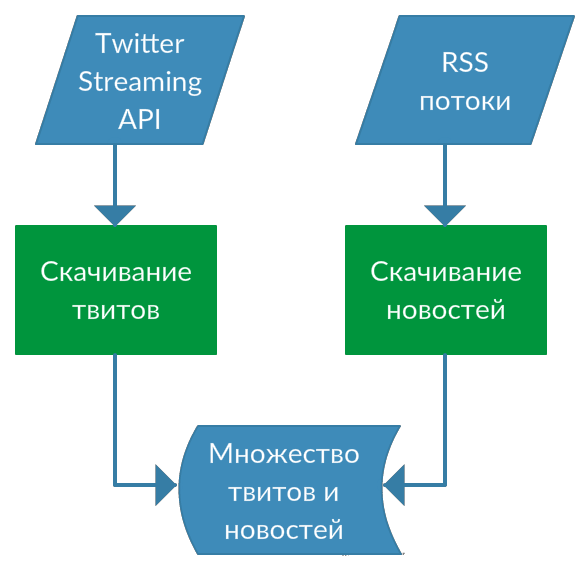
\includegraphics[scale=0.25]{twnews_consumer_flowchart.png}
            \caption{twnews consumer}
            \label{pic:consumer_flowchart}
    \end{figure}

    абзац про построение наборов данных

    абзац про векторы для сравнений

    абзац про получение моделей и векторов для сравнений датасетов

    абзац про метрики и рекомендации

    то-то изображено на рисунке~\ref{pic:twnews_flowchart_1}

    \begin{figure}[h!]
            \center
            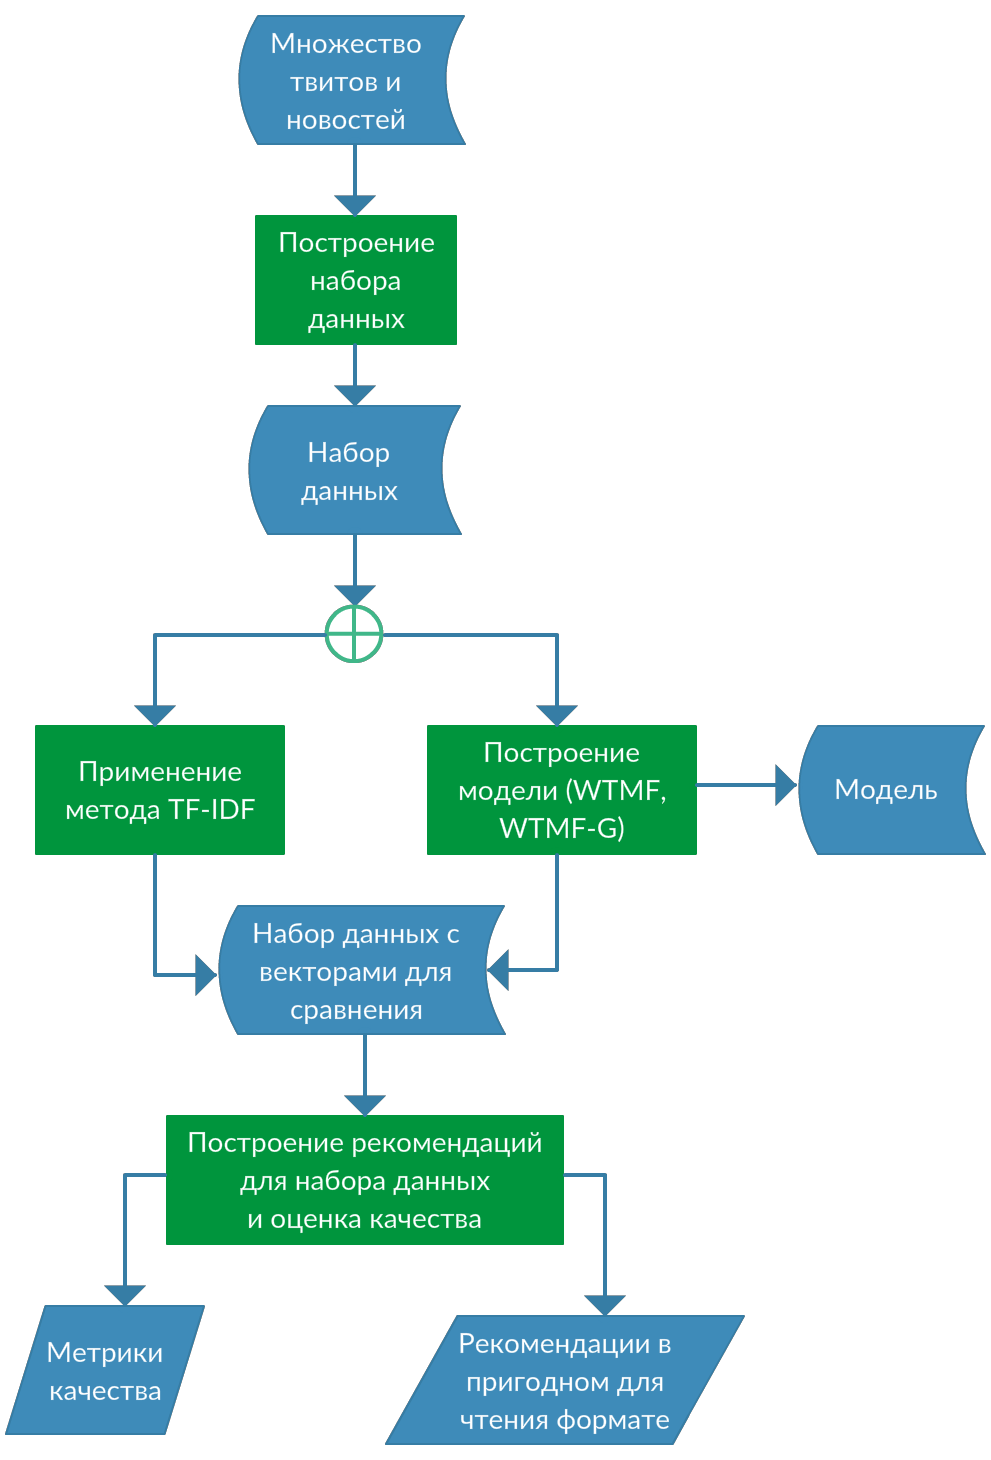
\includegraphics[scale=0.25]{twnews_flowchart_1.png}
            \caption{eval}
            \label{pic:twnews_flowchart_1}
    \end{figure}

    рекомендации для произвольных твитов строятся так-то

    то-то изображено на рисунке~\ref{pic:twnews_flowchart_2}

    \begin{figure}[h!]
            \center
            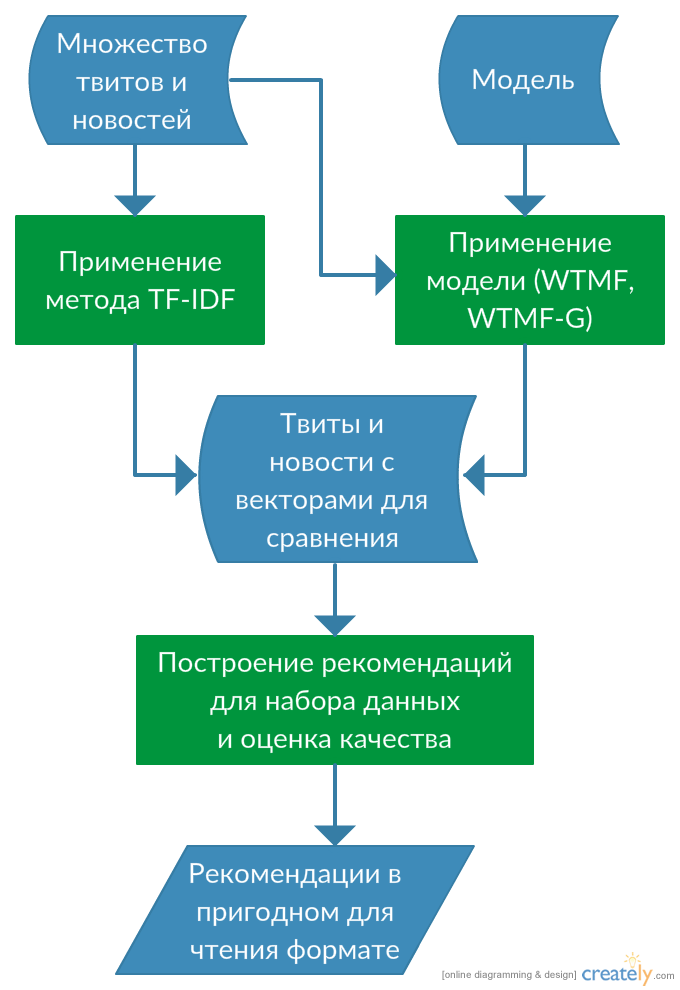
\includegraphics[scale=0.25]{twnews_flowchart_2.png}
            \caption{recommend}
            \label{pic:twnews_flowchart_2}
    \end{figure}

    абзац про завершение

    \clearpage



